% Created 2026-03-25 Wed 11:28
% Intended LaTeX compiler: pdflatex
\documentclass[11pt]{article}
\usepackage[utf8]{inputenc}
\usepackage[T1]{fontenc}
\usepackage{graphicx}
\usepackage{longtable}
\usepackage{wrapfig}
\usepackage{rotating}
\usepackage[normalem]{ulem}
\usepackage{amsmath}
\usepackage{amssymb}
\usepackage{capt-of}
\usepackage{hyperref}
\author{Gabriel G. de Brito}
\date{2026-03-24}
\title{Redux-Piá}
\hypersetup{
 pdfauthor={Gabriel G. de Brito},
 pdftitle={Redux-Piá},
 pdfkeywords={},
 pdfsubject={},
 pdfcreator={Emacs 30.2 (Org mode 9.7.11)}, 
 pdflang={English}}
\begin{document}

\maketitle
\tableofcontents

\section{Tabela de Instruções e sinais de controle}
\label{sec:orgd8f552f}
\begin{center}
\begin{tabular}{rlllrrrrrrrl}
Opcode & Mnemônico & Tipo & rw & ld & rwe & mwe & +pc & loop & b & acc & func\\
\hline
0000 & brzr & R & X & 0 & 0 & 0 & X & 0 & 1 & 0 & not\\
0001 & ji & I & X & 0 & 0 & 0 & +sI & 0 & 0 & 0 & X\\
0010 & ld & R & a & 1 & 1 & 0 & 1 & 0 & 0 & 0 & X\\
0011 & st & R & X & 0 & 0 & 1 & 1 & 0 & 0 & 0 & X\\
0100 & addi & I & 0 & 0 & 1 & 0 & 1 & 0 & 0 & 0 & add\\
0101 & ldui & I & 0 & 0 & 1 & 0 & 1 & 0 & 0 & 0 & ldui\\
0110 & loop & I & 3 & 0 & 1 & 0 & X & 1 & 0 & 0 & sub\\
0111 & mac & R & a & 0 & 1 & 0 & 1 & 0 & 0 & 1 & mul\\
1000 & not & R & a & 0 & 1 & 0 & 1 & 0 & 0 & 0 & not\\
1001 & and & R & a & 0 & 1 & 0 & 1 & 0 & 0 & 0 & and\\
1010 & or & R & a & 0 & 1 & 0 & 1 & 0 & 0 & 0 & or\\
1011 & xor & R & a & 0 & 1 & 0 & 1 & 0 & 0 & 0 & xor\\
1100 & add & R & a & 0 & 1 & 0 & 1 & 0 & 0 & 0 & add\\
1101 & sub & R & a & 0 & 1 & 0 & 1 & 0 & 0 & 0 & sub\\
1110 & slr & R & a & 0 & 1 & 0 & 1 & 0 & 0 & 0 & <<\\
1111 & srr & R & a & 0 & 1 & 0 & 1 & 0 & 0 & 0 & >>\\
\end{tabular}
\end{center}
\section{Sinais de controle}
\label{sec:orgf5976c9}
\begin{itemize}
\item Tipo: Se I, a entrada \texttt{ra} do banco de registradores deve receber 0; \texttt{rb}
deve receber 3. Se R, as entradas recebem o valor dos seus campos na
instrução. Se I, a entrada \texttt{b} da ula deve receber o imediato com sinal
extendido.
\item rw: Se a, a entrada \texttt{rw} do banco de registradores deve receber o valor do
campo ra da instrução. Se 0, deve receber 0. Se 3, deve receber 3.
\item ld: Se ativa, a entrada \texttt{d} do banco de registradores deve receber a saída
da memória.
\item rwe: Conectada diretamente à entrada \texttt{we} do banco de registradores.
\item mwe: Conectada diretamente à entrada \texttt{mwe} da memória.
\item +pc: Se +sI, o PC deve ser somado ao imediato com sinal. Se -uI, deve
ser decrementado do imediato somado à 1 sem sinal. Se 1, deve ser somado
à 1.
\item loop: Se ativa, a entrada \texttt{a} da ula deve ser -1. Caso o resultado da ula
seja diferente de zero, PC deve receber a subtração de si próprio pelo
imediato sem sinal + 1.
\item b: Se ativa e a saída da ula for diferente de 0, o PC deve ao invés da
soma, receber o valor da saída \texttt{b} do banco de registradores.
\item acc: Conectada diretamente à entrada \texttt{acc} do banco de registradores.
\item func: Função a ser computada na ula.
\end{itemize}
\subsection{Codificações}
\label{sec:org1bd915e}
\begin{itemize}
\item Tipo: 1 bit, R = 0, I = 1.
\item rw: 2 bits, a = 0, 0 = 1, 3 = 2.
\item +pc: 1 bit, 1 = 0, +sI = 1.
\item func: 4 bits:
\begin{itemize}
\item add = 0.
\item sub = 1.
\item not = 2.
\item and = 3.
\item or = 4.
\item xor = 5.
\item << = 6.
\item >> = 7.
\item mul = 8.
\item ldui = 9.
\end{itemize}
\end{itemize}
\section{Instruções extendidas}
\label{sec:orga1af1e2}
\subsection{loop}
\label{sec:orgbecf823}
A instrução decrementa o registrador \texttt{r3} e, caso o resultado seja diferente
de zero, desvia o programa subtraindo o imediato sem sinal + 1 do PC.
\subsection{mac}
\label{sec:orgf059d2f}
A instrução multiplica os valores de \texttt{ra} e \texttt{rb}, guardando o resultado em \texttt{r0}.
\subsection{ldui}
\label{sec:orge66483c}
A instrução concatena a parte baixa de \texttt{r0} com o imediato na parte alta.
\section{Notas do projeto}
\label{sec:orga5d6c9d}
\subsection{\texttt{acc}}
\label{sec:org8a8f230}
O banco de registradores possui uma entrada adicional \texttt{acc} que, caso ativa,
soma o valor a ser guardado no registrador ao invés de substituí-lo.
\section{Diagramas}
\label{sec:org442dde9}
\begin{figure}[htbp]
\centering
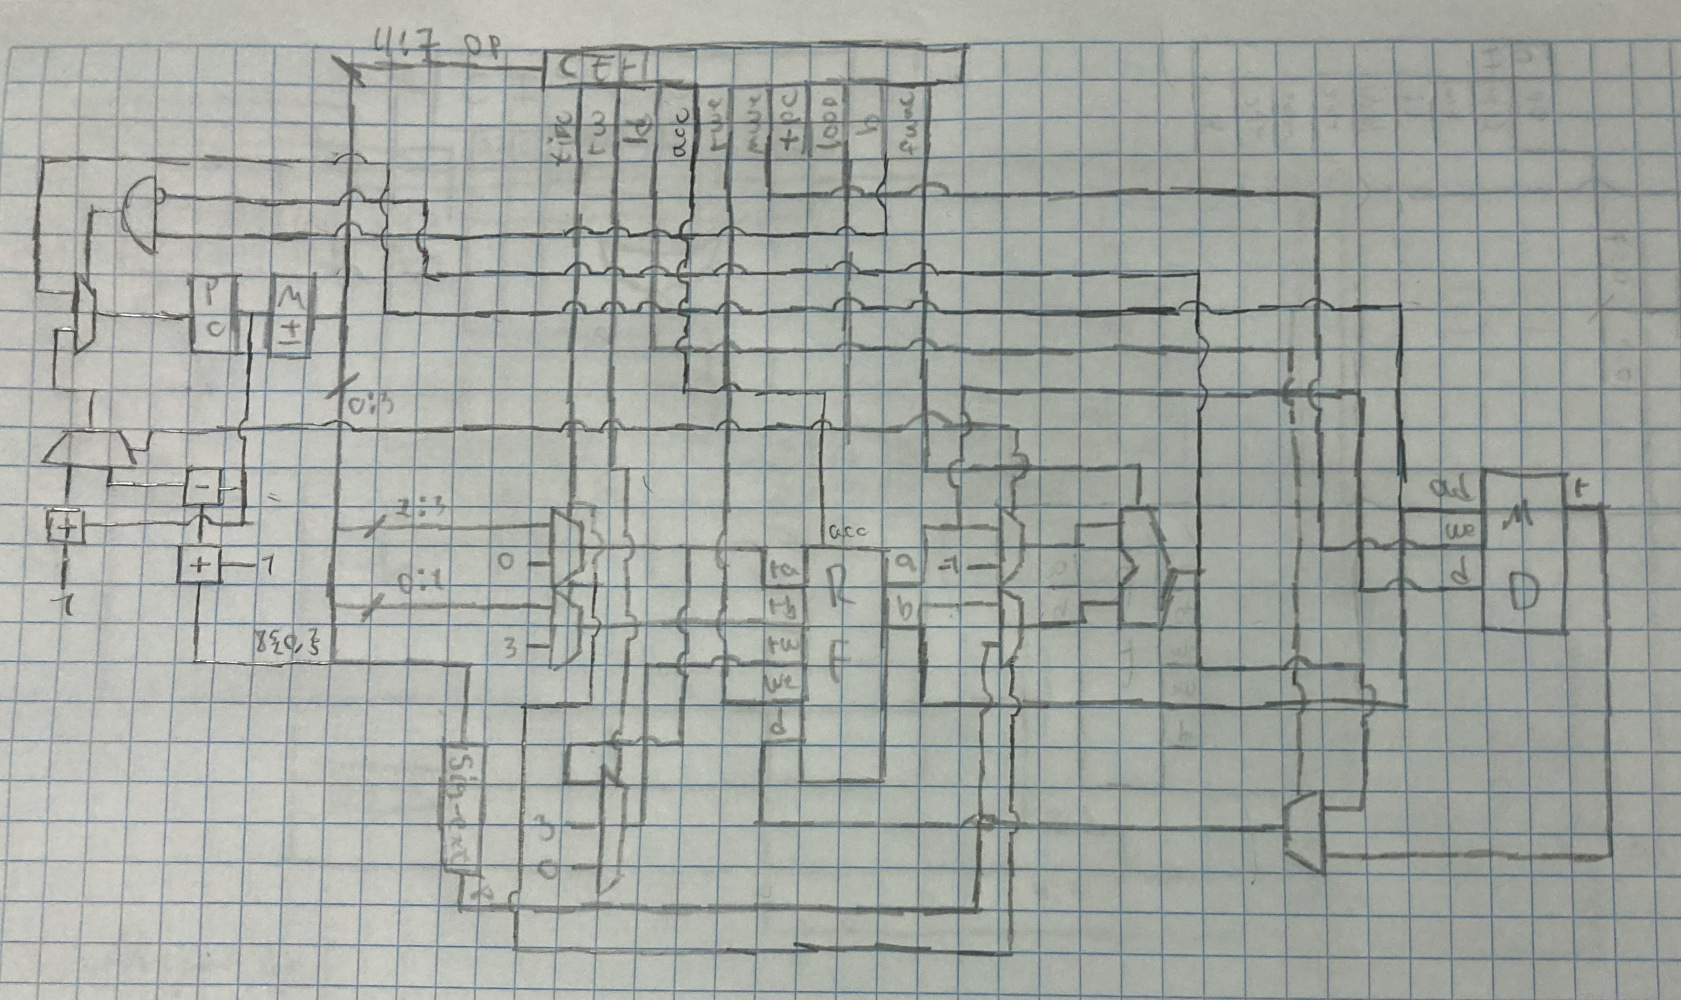
\includegraphics[width=.9\linewidth]{./redux-pia/redux.jpg}
\caption{Diagrama do REDUX-PIÁ.}
\end{figure}

\begin{figure}[htbp]
\centering
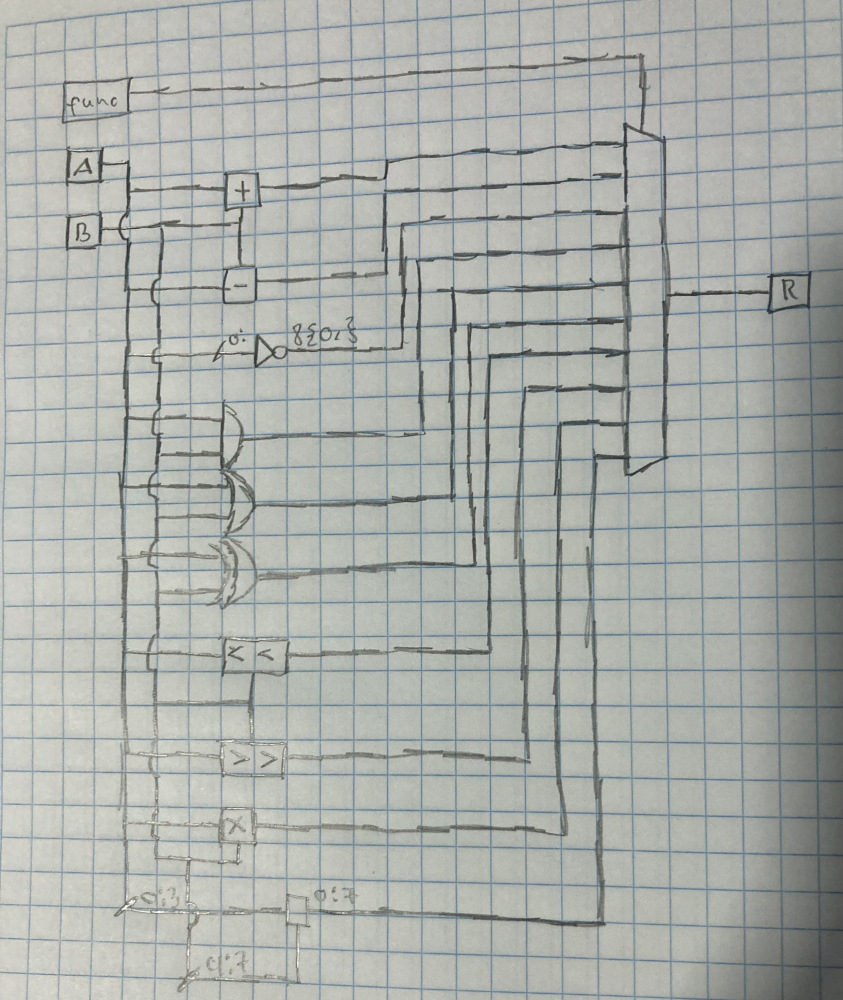
\includegraphics[width=.9\linewidth]{./redux-pia/ula.jpg}
\caption{Diagrama da ula.}
\end{figure}
\section{Assembly}
\label{sec:org9a7b2cf}

O programa que faz soma vetorial:

\begin{verbatim}
        xor r0, r0
        xor r1, r1
        xor r2, r2
        xor r3, r3

        addi 5
        addi 5

        add r1, r0

        xor r0, r0
        addi 7
        ldui 1

        add r2, r0

        xor r0, r0
        addi 3

        add r3, r0
        xor r0, r0
        addi 1
for:
        st r1, r2

        add r1, r0
        add r2, r0

        loop for

        xor r0, r0
        addi 1
;; ji 0
        ecall
\end{verbatim}

O programa que faz produto escalar de dois vetores:

\begin{verbatim}
        xor r0, r0
        xor r1, r1
        xor r2, r2
        xor r3, r3

        addi 5
        add r3, r0

        xor r0, r0
for:
;; Por conveniência, vamos usar a posição 0 da memória para guardar o
;; acumulador. Esse loop tem exatamente o tamanho limite para usar a instrução
;; loop.
        xor r1, r1
        st r0, r1

        xor r0, r0
;; Os vetores ficam em 0x20 para salvar uma instrução aqui e manter o loop no
;; tamanho para utilizar a instrução loop.
        ldui 2
        add r0, r3
        xor r2, r2
        add r1, r0
        add r2, r0
        xor r0, r0
        addi 5
        add r2, r0
        ld r1, r1
        ld r2, r2

        xor r0, r0
        ld r0, r0

        mac r1, r2

        loop for

        xor r0, r0
        addi 1
;; ji 0
        ecall

.space 5
a:
.bits8 1
.bits8 2
.bits8 3
.bits8 4
.bits8 5
b:
.bits8 5
.bits8 4
.bits8 3
.bits8 2
.bits8 1
\end{verbatim}
\end{document}
